
%%%%%%%%%%%%%%%%%%%%%%%%%%%%%%%%%%%%%%%%%%%%%%%%%%%%%%%%%%%%%%%%%%%%%%%%%%%%%%%
%
% Nicole's Thesis, IIT 2018
%
%%%%%%%%%%%%%%%%%%%%%%%%%%%%%%%%%%%%%%%%%%%%%%%%%%%%%%%%%%%%%%%%%%%%%%%%%%%%%%%
\documentclass{iitthesis}

% Document Options:
%
% Note if you want to save paper when printing drafts,
% replace the above line by
%
%   \documentclass[draft]{iitthesis}
%
% See Help file for more about options.

\usepackage{graphicx}    % This package is used for Figures
\usepackage{rotating}           % This package is used for landscape mode.
\usepackage{epsfig}
\usepackage{subfigure}          % These two packages, epsfig and subfigure, are used for creating subplots.
\usepackage{siunitx}
\usepackage[shortcuts]{extdash}
\renewcommand{\thefootnote}{\arabic{footnote}}
\usepackage[bf, labelsep=period]{caption}
\usepackage{url}
\usepackage{booktabs}
\usepackage[american]{circuitikz}
\usepackage[normalem]{ulem}

\usepackage{tikz}
\usetikzlibrary{shapes.misc}
\usetikzlibrary{shapes,arrows,decorations.markings,shadows,positioning}

%% Only for editing process...TAKE OUT for FINAL DRAFT
\usepackage{graphicx,xcolor,enumitem}
\newcommand{\lsnote}[1]{\textsf{{\color{violet}{ LS note:}   #1 }}}
\newcommand{\nrnote}[1]{\textsf{{\color{blue}{ NN note:}   #1 }}}
\newcommand{\jpnote}[1]{\textsf{{\color{green}{ JP note:}   #1 }}}


%Code formatting???
\usepackage[utf8]{inputenc}
\usepackage{listings}
\usepackage{color}

\definecolor{codegreen}{rgb}{0,0.6,0}
\definecolor{codegray}{rgb}{0.5,0.5,0.5}
\definecolor{codepurple}{rgb}{0.58,0,0.82}
\definecolor{backcolour}{rgb}{0.95,0.95,0.92}

\lstdefinestyle{mystyle}{
	backgroundcolor=\color{backcolour},   
	commentstyle=\color{codegreen},
	keywordstyle=\color{magenta},
	numberstyle=\tiny\color{codegray},
	stringstyle=\color{codepurple},
	basicstyle=\footnotesize,
	breakatwhitespace=false,         
	breaklines=true,                 
	captionpos=b,                    
	keepspaces=true,                 
	numbers=left,                    
	numbersep=5pt,                  
	showspaces=false,                
	showstringspaces=false,
	showtabs=false,                  
	tabsize=2
}

\lstset{style=mystyle}

\begin{document}

\title{Design for Staged Two Beam Acceleration at the Argonne Wakefield Accelerator Facility}

\author{Nicole Neveu }
\degree{Doctor of Philosophy}
\dept{Physics}
\date{May 2018}
\copyrightnoticetrue      % crate copyright page or not
%\coadvisortrue           % add co-advisor. activate it by removing % symbol to add co-advisor
\maketitle                % create title and copyright pages


\prelimpages         % Settings of preliminary pages are done with \prelimpages command

%%%  Acknowledgement %%%
\begin{acknowledgement}     % acknowledgement environment, this is optional
	\par  Family, Lalo, Linda, John, AWA group, Jeff
	%\input{ackno.tex} % you need a separate acknowledgement.tex file to include it.
\end{acknowledgement}

% Table of Contents
\tableofcontents
\clearpage

% List of Tables
\listoftables
\clearpage

%List of Figures
\listoffigures
\clearpage

%List of Symbols(optional)

\listofsymbols
\SymbolDefinition{$c$}{Speed of Light}
\SymbolDefinition{$\epsilon$}{Dielectric Permittivity}
\SymbolDefinition{$\epsilon$}{6D Phase Space Emittance}
\SymbolDefinition{$\gamma$}{Relativistic Kinetic Energy}

\clearpage

%%% Abstract %%%
\begin{abstract}           % abstract environment, this is optional
	\par Staged two beam acceleration using dielectric structures has yet to 
	be achieved anywhere in the world. In this thesis, I discuss the beam 
	line design and simulation, followed by experimental results of a 
	beam line with the potential for dielectric TBA.   
\end{abstract}

\textpages     % Settings of text-pages are done with \textpages command

\Chapter{INTRODUCTION}
%%%%%%%%%%%%%%%%%%%%%%%%%%%%%%%%%%%%%%%%%%%%%%%%%%%%%%%%%%%%%%%%%%%%%%%%%%%%%%%%%%%%%%%%%%%%
%%%%%%%%%%%%%%%%%%%%%%%%%%%%%%%%%%%%%%%%%%%%%%%%%%%%%%%%%%%%%%%%%%%%%%%%%%%%%%%%%%%%%%%%%%%%
\Section{Motivation} \label{sec:motivation}
%%%%%%%%%%%%%%%%%%%%%%%%%%%%%%%%%%%%%%%%%%%%%%%%%%%%%%%%%%%%%%%%%%%%%%%%%%%%%%%%%%%%%%%%%%%%
%%%%%%%%%%%%%%%%%%%%%%%%%%%%%%%%%%%%%%%%%%%%%%%%%%%%%%%%%%%%%%%%%%%%%%%%%%%%%%%%%%%%%%%%%%%%
A new generation of accelerators dedicated to High Energy Physics
(HEP), would likely be of the TeV scale. Reduction in the size and cost
of such machines is key to their feasibility, and can be accomplished
through accelerator technology R\&D. Investigation into a 
high gradient candidate for future HEP machines is an active research area
at the Argonne Wakefield Accelerator (AWA) facility. A
short pulse, two-beam acceleration (TBA) scheme using 
wakefield power extractors, and accelerating structures made 
of metallic materials was demonstrated~\cite{recent-tba}. 
A goal of the AWA group is to demonstrate fully staged TBA, 
achieving a gradient of 250 MV/m. If successful, this would
be the only facility in the world capable of such gradients used for
acceleration of a beam.

TBA requires a drive beam to pass through a decelerating structure and
loss of energy through wakefield generation. The electromagnetic wake
is coupled from the decelerator into an accelerating structure, where
the electric field is used to accelerate a second beam. In order to have equivalent power 
generation for each stage, two complete and separate beamlines 
operating synchronously with each other are required.  
The wakefield structures can be metallic or dielectric. Dielectric
structures, having no irises, are simple to manufacture and have demonstrated
high gradient capability at \SI{100}{MV/m} \cite{WeiPaper}. 

The Compact Linear Collider (CLIC) collaboration, proposes a similar TBA scheme with
a \SI{240}{ns} pulse design. This limits the acceleration gradient
to roughly \SI{150}{MV/m} at room temperature due to rf breakdown \cite{CLICdesignReport}.
Higher gradients could be reached when driven by a very short drive
beam pulse, such as the 20ns pulse length proposed by AWA \cite{WeiPaper}. 
\nrnote{Understand and explain why short pulse can give higher gradients. 
Because higher peak power is tolerable, but average power stays the same?}
While the two groups vary on approach, they agree that TBA would 
require less infrastructure when constructing a linear TeV scale machine, 
versus the cost of more conventional technology. 
For example, a case study was done comparing the infrastructure 
needed when using traditional \SI{50}{MW} klystron sources.
It would take roughly 35,000 klystrons to construct a linear machine to deliver the same 
\SI{9.2}{TW} power as in the CLIC design specification in CLIC reports \cite{CLICdesignReport}. 
In comparison to CLIC's 48 km projected machine length needed to reach \SI{3}{TeV}, the Next Linear
Collider (NLC) collaboration projected a machine length of \SI{26}{km} using X-band klystrons,
only to reach an energy of \SI{1}{TeV}. %\cite{NLC}. 
\lsnote{The text below is not well developed.  I guess since it is in this paragraph, you are trying to explain the statement that less infrastructure is required.  First, you don't say anything specifically about using an accelerator beam rather than a klystron - how does that save on equipment and space?  It is also confusing that you start by saying the power to the witness beam is conventional, abut then say there is a difference in infrastructure with nothing between  about why.}
The power supplied to the witness beam in TBA is similar to
power provided by traditional accelerator technology. 
The key difference is the amount of infrastructure and cost 
needed to transport the power. Theoretically, TBA can deliver
the same amount of power as conventional methods with less 
infrastructure, and therefore lower cost, in the case of a high energy machine. 

\lsnote{This next section of text should be a summary of what was done for your thesis, what the results were, and why they were important. Perhaps mapping them to the corresponding sections of your thesis.  The AWA facility and following sections should probably be in the next chapter.  You probably can't write these paragraphs until finishing your work.}

Before a detailed understanding of the power and infrastructure trade offs 
can be obtained, the feasibility of staged TBA must be be demonstrated as viable, 
as no high energy machine can be built without staging.
Staging is the ability to use two successive accelerating modules to synchronously accelerate 
the same particle bunch. While simple in principle, the difficulties 
in achieving staging should not be underestimated. 
Demonstration of staging proves that a TBA scheme can be scaled to high energies, and whether it is 
feasible to use such methods. Single stage TBA, and staging 
in a simplified scheme have been demonstrated at the AWA in 2016.
\nrnote{Not any more? - Demonstration of the full-scale dielectric staging scheme is the 
	subject of this thesis.} 
Desing and partial testing of a full-scale staging scheme is the 
subject of this thesis. The branched drive beam line was designed and 
simulated. 
Optimization of the bunch train timing took place, \nrnote{not? - the two 
	beam lines were synchronized and experimental measurements 
	of staged TBA were taken. }
Experimental results and comparison to simulations, along 
with the following beam dynamics analysis is shown here.

%%%%%%%%%%%%%%%%%%%%%%%%%%%%%%%%%%%%%%%%%%%%%%%%%%%%%%%%%%%%%%%%%%%%%%%%%%%%%%%%
%%%%%%%%%%%%%%%%%%%%%%%%%%%%%%%%%%%%%%%%%%%%%%%%%%%%%%%%%%%%%%%%%%%%%%%%%%%%%%%%
\Section{Argonne Wakefield Accelerator Facility} \label{sec:facility}
%%%%%%%%%%%%%%%%%%%%%%%%%%%%%%%%%%%%%%%%%%%%%%%%%%%%%%%%%%%%%%%%%%%%%%%%%%%%%%%%
%%%%%%%%%%%%%%%%%%%%%%%%%%%%%%%%%%%%%%%%%%%%%%%%%%%%%%%%%%%%%%%%%%%%%%%%%%%%%%%%

\iffalse
\nrnote{this paragraph is from NAPAC paper}
The AWA facility houses a 70 MeV RF photoinjector \cite{upgrades} with a large 
dynamic range: 20 pC to 100 nC. In many cases, the beam is SC dominated. 
In the AWA’s Emittance Exchange (EEX) beam line \cite{eex}, CSR has a large  
effect on the beam as it passes through the dipoles, and wakefields
are present in the two beam acceleration (TBA) beam line \cite{staging1}. ASTRA, 
GPT, and OPAL-T are capable of simulating 3D SC, and wakefield effects.
The latter two codes also include a CSR model, making them a good fit for the AWA.  
\fi

The AWA facility houses two rf photoinjector electron guns operating
at \SI{1.3}{GHz}, and three subsequent beam lines. 
Two of the beam lines are currently used for staged TBA, and the
third is used for Emittance Exchange experiments (EEX). A layout of
the facility is shown in Fig. \ref{fig:bunker}. 
\lsnote{Some more detail will be needed here, maybe just switch the order of the some of the text in the two paragraphs below.  Something like; start with saying what the beamlines are and what is in them referring to the figure, then describe their sources in more detail (RF guns and photocathodes), then talk about the laser and how it is split.}

Electron bunches in a photoinjector are created through the photoelectric effect. 
At the AWA, a pulsed UV laser is propagated through two relay lines of UV optics to either
the drive or witness gun. An in-vacuum mirror then directs the pulse to the photocathode.
Both beam lines must be operated simultaneously when the TBA experiments are run. This is accomplished by
splitting the original laser pulse into two pulses using a UV splitter on the 
ceiling of the bunker. One of the split pulses is sent (as is) to the witness beam line for one
bunch operation. The second pulse is sent to a UV multispitter table, shown in 
Fig.~\ref{fig:optics} where it is split into trains of various lengths. Eight pulses are 
used for TBA drive trains, 

The beam line located on the right side of Fig. \ref{fig:bunker} is called the
drive line. The rf photoinjector on the drive line uses a semiconducting
CsTe cathode, and is followed by a linear accelerator (linac). The
drive linac uses six copper cavities and four klystrons to accelerate the drive beam
to energies of 50-\SI{70}{MeV}. The number of bunches generated from each 
laser pulse can vary from 1, 2, 4, 6, and 8 bunches. When multiple bunches
are generated, the grouping is called a bunch train. Generation of
these variable bunch trains is accomplished by splitting the pulsed
UV laser beam before it enters the gun and hits the cathode. The splitting
takes place in a complex network of UV optics located near the drive
gun. The optics set up is called a beam splitter, or mulitsplitter,
and trains are created at a rate of 0.5, 1, or \SI{2}{Hz}. This timing is
called a pulse, or the repetition rate of the machine. A picture of
the AWA multisplitter table is shown in Fig. \ref{fig:optics}. Optimization 
of the UV optics was performed and is detailed in Section \ref{sec:uvoptics}.  

\iftrue
\begin{figure}
	\begin{center}
		%\includegraphics[width=\linewidth]{images/quads1}
		\label{fig:bunker}
	\end{center}
\end{figure}
\begin{figure}[h]
	\begin{center}
		\includegraphics[width=0.5\textwidth]{images/multisplitter}\caption{UV multisplitter optics table.}
	\end{center}
	\label{fig:optics}
\end{figure}
\fi

The witness line rf photoinjector, located on the left side of Figure
1, uses a Mg cathode and the following linac consists of one copper
accelerating cavity. Prior to the multisplitter table, shown in
Fig. \ref{fig:optics}, the laser pulse is split between the drive and witness side.
This set up allows only one bunch per pulse on the witness line. Also
note that the beam from the drive line travels in the opposite direction
than the beam in the witness line. 

%%%%%%%%%%%%%%%%%%%%%%%%%%%%%%%%%%%%%%%%%%%%%%%%%%%%%%%%%%%%%%%%%%%%%%%%%%%%%%%%%%%%%%%%%%%%
%%%%%%%%%%%%%%%%%%%%%%%%%%%%%%%%%%%%%%%%%%%%%%%%%%%%%%%%%%%%%%%%%%%%%%%%%%%%%%%%%%%%%%%%%%%%
\Section{Dielectric Structures}

%%%%%%%%%%%%%%%%%%%%%%%%%%%%%%%%%%%%%%%%%%%%%%%%%%%%%%%%%%%%%%%%%%%%%%%%%%%%%%%%%%%%%%%%%%%%
%%%%%%%%%%%%%%%%%%%%%%%%%%%%%%%%%%%%%%%%%%%%%%%%%%%%%%%%%%%%%%%%%%%%%%%%%%%%%%%%%%%%%%%%%%%%
\Subsection{Power Generation}

\lsnote{Somewhere you need a comprehensive description of simplified staging vesus full staging.  I am not sure it is here, but it should be before you mention simplified staging.}

Currently, all \lsnote{define PETS acronym} PETS and accelerating structures installed in the AWA's
simplified staging scheme are metallic. It has been shown that a few
key equations can demonstrate the relationship between beam parameters
and the resulting \lsnote{\sout{rf} power} generated in the decelerating cavity. This section
borrows heavily from previous work at CLIC and the AWA \cite{key-3,key-8}. 
Starting with the timing, each bunch in the drive train will generate
an rf pulse of finite length in the structure. Each bunch is separated
in time by $T_{b}$, and the \lsnote{average?} beam current can be written as $I=\frac{Q}{T_{b}}$.
\lsnote{define Q, is it the charge per bunch?} The bunches are Gaussian in the longitudinal direction, and the form
factor, $\Phi$, is used to describe\lsnote{\sout{s}} the Gaussian shape by taking
the Fourier transform of the charge distribution: 
\begin{equation}
\Phi=exp\left[\frac{-(k_{z}\sigma_{z})^{2}}{2}\right]
\end{equation}
Where $k_{z}=\frac{2\pi}{\lambda_{z}}$ is the longitudinal wave number
and $\sigma_{z}$ is the rms bunch length. \lsnote{That was confusing.  You said phi was the FT of the charge distribution, but in the equation after that it looks like the charge distribution not the FT}  Note the subscript z \lsnote{indicates \sout{refers to the characteristics of the cavity and bunch in}} the longitudinal
direction. Then using the partial differential equation that relates
the power generated by the wakefield to the change in power over time, \lsnote{I would include the equation}
the power generated by a bunch train can be written as:
\begin{equation} \label{eq:rfpower}
P_{t}(t)=\frac{\omega_{z}\,L^{2}I^{2}}{4\,v_{g}}\frac{R}{Q_{d}}\left(\frac{1-e^{-\alpha L}}{\alpha L}\right)\Phi^{2}
\end{equation}
With $I$ being the beam current as defined above, $\alpha=\frac{\omega}{2Q_{d}v_{g}}$
being the attenuation constant \cite{key-9}, R is the shunt impedance
per unit length, and $Q_{d}$ is the quality factor for the decelerating
structure. \lsnote{You didn't define L or vg} Note, the derivation of equation 4 can be found in reference
\cite{key-8}, and due to the complex geometry of metallic structures,
the value of R/Q is often calculated in electromagnetic codes such
as CST Microwave Studio. 

\lsnote{You probably were intending to do this, but this section should close out with a predicted power generation 
in the decelerating structures.  The discussion of how that depends on number of bunches in the bunch train should be here as well.}

\Subsection{Accelerating Structures}

\Section{Two Beam Acceleration}

\Section{AWA Design Requirements} \label{sec:requirements}

\lsnote{This is probably where you should have the overview of simple staging versus full staging, and a summary of what was required to go to full staging.  The title of the section should also be changed, maybe `Fully staged two beam acceleration'?}

In order to design and test the desired beam line, three technologies 
new to the AWA were investigated. These include a kicker, septum magnets, 
and non-GA optimization algorithms.

% An example for enumerate
\begin{enumerate}
	\item Kicker Design
	\item Septum Design
	\item Optimization 
\end{enumerate}

% A quotation example
% Every quota must be accompanied by a reference to the source
% in a footnote or in the Bibliography
\begin{quotation}
	test
\end{quotation}

\clearpage


\Chapter{Experimental Set Up}
Before final measurements or meaningful simulations can be done, 
a fair amount of set up and preliminary measurements 
must be made and understood. 

%%%%%%%%%%%%%%%%%%%%%%%%%%%%%%%%%%%%%%%%%%%%%%%%%%%%%%%%%%%%%%%%%%%%%%%%%%%%%%%%%%%%%%%%%%%%
%%%%%%%%%%%%%%%%%%%%%%%%%%%%%%%%%%%%%%%%%%%%%%%%%%%%%%%%%%%%%%%%%%%%%%%%%%%%%%%%%%%%%%%%%%%%
\Section{Laser Pulse Train Improvement} \label{sec:uvoptics}
%%%%%%%%%%%%%%%%%%%%%%%%%%%%%%%%%%%%%%%%%%%%%%%%%%%%%%%%%%%%%%%%%%%%%%%%%%%%%%%%%%%%%%%%%%%%
%%%%%%%%%%%%%%%%%%%%%%%%%%%%%%%%%%%%%%%%%%%%%%%%%%%%%%%%%%%%%%%%%%%%%%%%%%%%%%%%%%%%%%%%%%%%

Ideally, to extract maximum power from a series of bunches, each electron bunch should have the same amount of charge.  Improving the laser pulse train intensity distribution improves the electron bunch charge distribution; 
which  helps produce an RF power pulse that is closer to uniform. 
The generated power depends on both the charge and shape of the bunch, as shown in Eq.~\ref{eq:rfpower}. 
Several factors contribute to non-uniformity in the bunches. These include the cathode material
(i.e. slightly different QE along the surface), shot to shot noise in the laser pulse, 
distortion of laser pulses due to traveling through air, and the quality of the optics. 
The last is especially important in determining the intensity of each laser pulse in the train.  
Each splitter has a slightly different value for transmitted (T) and reflected (R) pulses. 

\Subsection{UV Optics} 
In order to generate the drive bunch trains needed for TBA, a UV laser pulse is split 
by five optical splitters into two trains of eight pulses. 
The optics set up is shown in Fig~\ref{fig:optics}. Optical delay lines (two mirrors) near each splitter 
separate pulses in space and time by extending the distance that each pulse travels. 
The length of each delay line is a multiple of the RF frequency, 1.3 GHz. 
In other words, a separation of $1\lambda=\SI{769}{ps}$ between each UV pulse is created. 
This is done to synchronize the laser pulses with the RF supplied to the gun.
In order to achieve equally charged bunches, splitters with a perfect transmission 
to reflection ratio ($T/R = 50/50$) would be required.

\Subsection{UV Splitter Measurements} 
The initially installed splitters were rated at a tolerance of $50\%\pm5\%$.
Measurements of the UV splitters were done to determine the T/R (Transmission to Reflection) ratio for 
each splitter. The measurements took place in the laser room, close to the source of the laser.
The setup included two joule meters; one to measure the raw T/R values and one to measure 
the background. Amplified Spontaneous Emission (ASE), 
is the main contributor to background shot to shot noise in the laser pulse,
and is known to drift with temperature and operating time. 
The ASE value was measured when each T/R measurement was taken, then divided out of the T/R 
measurements to prevent bias due to background drifts. 

Several configurations were tested this way: S-polarization, P-polarization, 
and laser incident on back or front of the coating. 
Whether the laser pulse hit the front or back of the optic
had no measurable effect on the T/R ratio. Polarization did have a significant effect on
the results, which led to more careful observation of this in the future.
The following plot shows the splitters were performing at about 55/45 ratio, 
The results indicated the ratio of reflection to transmission for each splitter ranged from 
$T/R\approx55/45$ to $53/47$. 
This caused an uneven laser intensity distribution, as the bunch intensity depends on the path 
it takes through the multisplitter optics. Pulses that were reflected more than one
time could have significantly lower intensities than other bunches. 
Consider the path of laser pulse four as shown in Fig.~\ref{fig:tikz}. 
The pulse is transmitted through splitters 1, 2, and 4, but is reflected by splitter 3.
\def \delayvertical {1.5}
\def \delayoneleft {7.5}
\def \delaytworight{15}
\def \mycenter{10.0}
\def \labels{6.5}
\def \sone {-0.5}
\def \stwo {\sone+1.5}
\def \sthree {\stwo+1.5}
\def \sfour {\sthree+1.5}
\def \buffer{-4.5}
\iffalse
\begin{figure*}[h]
	\begin{center}		
		\begin{tikzpicture}[scale=0.7]
		%\node[] at (\labels, 5.5) {Behavior through splitter};
		\node[] at (\labels,6.0) {$T$};
		\node[] at (\labels,4.5) {$T$};
		\node[] at (\labels,3.0) {$R$};
		\node[] at (\labels,1.5) {$T$};
		\node[] at (\labels,0.0) {$T$};
		
		\draw[very thick] (10.5,\sone) -- (9.5,\sone+1); % Splitter 1
		\draw[very thick] (10.5,\stwo) -- (9.5,\stwo+1); % Splitter 2
		\draw[very thick] (10.5,\sthree) -- (9.5,\sthree+1); % Splitter 3
		\draw[very thick] (10.5,\sfour) -- (9.5,\sfour+1); % Splitter 4
		
		\draw[cyan, very thick] (\delayoneleft,0.0) -- (20.0,0.0) % Incoming pulse line
		to(\delayoneleft,0.0) -- (\delayoneleft,\delayvertical) % Delay Leg 1 (a)
		to(\delayoneleft,\delayvertical) -- (15,\delayvertical); % Pulse after delay 1
		
		\draw[cyan,very thick] (\mycenter,\delayvertical*2) -- (\delaytworight,\delayvertical*2)
		to(\delaytworight,\delayvertical) -- (\delaytworight,\delayvertical+1.5)
		to(\mycenter,\delayvertical*2) -- (\mycenter,\delayvertical*4);
		
		\draw[cyan, very thick] (9.7,5.5) -- (10.0,6.0); % arrow head left
		\draw[cyan, very thick] (10.0,6.0) -- (10.3,5.5); % arrow head right
		
		\node[] at (18,0.5) {Laser pulse};
		
		\node[] at (8.75,-1.7) {$1\lambda$};
		\draw[black, very thick] (\delayoneleft, -1) -- (\delaytworight, -1);
		\draw[black, very thick] (\delayoneleft, -1.5) -- (\delayoneleft, -0.5);
		\draw[black, very thick] (\mycenter, -1.5) -- (\mycenter, -0.5);
		
		\node[] at (12.5,-1.7) {$2\lambda$};
		\draw[black, very thick] (\delaytworight, 3.0+\buffer) -- (\delaytworight, 4.0+\buffer);
		
		\end{tikzpicture}
	\end{center} 
	\caption{Example of a laser pulse path through multisplitter. T indicates when the laser pulse is 
		transmitted through the splitter, and R stands for when the laser pulse is reflected by the splitter. 
		The operating wavelength is $\lambda = \SI{23}{cm}$. Bends are accomplished with two UV mirrors, 
		one at each corner of the delay line.}
	\label{fig:tikz}
\end{figure*}
\fi

Each splitter reduces the intensity of the pulse as a new pulse is generated. Expected intensities
can be predicted by using the measured T/R values for each splitter. For example, using $T/R=55/45$,
in Fig~\ref{fig:tikz} the laser pulse is transmitted four times and reflected once: 
\begin{equation}\label{eq:i4}
I_4 =  T \cdot R \cdot T \cdot T \cdot T \cdot I_0 \approx 0.41 I_0
\end{equation}
Therefore, this pulse had a fairly high laser intensity, because it was transmitted multiple times. 
In the worst case, the laser intensity of pulse six: 
\begin{equation}\label{eq:i6}
I_6 =  T \cdot R \cdot R \cdot R \cdot T \cdot  I_0 \approx 0.28 I_0
\end{equation}
These trends were reflected in the electron bunch trains generated in the gun.
As a result, methods to improve the intensity distribution were investigated.

\Subsection{New UV Splitters}
To improve the intensity distribution, splitters with a tolerance of $50\%\pm3\%$ were purchased, 
installed, and the laser energy was measured again. The quality of the splitters was near tolerance 
again, and the bias leaned toward reflection, $T/R \approx 47/53$. With the bias now reversed, 
the trend in intensity distribution was also reversed. The possibility of using a combination 
of splitters from the $\pm3\%$ and $\pm5\%$ sets was explored. 
Using a python script to compare all possible combinations, it was determined that using only 
$\pm3\%$ splitters would result in the lowest variation in intensity. 

\Subsection{Train Intensity Measurements}
To verify the predictions above, and show improvement using the $\pm3\%$,
the intensity of bunches one through eight were measured using four splitters. 
This simplified the experimental set up, and reduced interruption to beam time 
runs which were using the four splitter set up.  
\iffalse
\begin{figure}[h]
	\begin{center}
		\includegraphics[width=0.8\textwidth]{images/splitter_improvement}\caption{Laser pulse train intensity measurements}
	\end{center}
	\label{fig:origtrain}
\end{figure}
\fi
The predictions in Eqs.~\ref{eq:i4} and~\ref{eq:i6} don't account for mirror losses in the delay legs, 
so we expect a lower value in experiment. To do a quick check on whether or not these results are 
expected, consider laser pulse one and only four splitters (as was the experimental set up). 
Laser pulse one has a similar path to laser pulse four (Eq.~\ref{eq:i4}). 

\begin{equation}
I_1 = R \cdot T \cdot T \cdot T \cdot I_0 
\end{equation}

Given about $\pm10\%$ mirror loss in the delay legs, we expect laser pulse one and four 
to be roughly the same intensity. This is shown in Fig.~\ref{fig:origtrain}. With the same 
logic, we expect pulse six to have the largest deviation from pulse one, as it is reflected 
three times and transmitted once in the four splitter set up. This expectation is also 
confirmed by the results in Fig.~\ref{fig:origtrain}.  \lsnote{You achieved a significant improvement in the uniformity of the laser pulse train, as can be seen in the figure.  Even though it can be seen in the figure, you should wrap up the section with a quantitative statement about the improvement you achieved, along with a summary sentence on how you achieved it.  Something like, `Through the use of optics with tighter specifications, and sorting of the optical elements, an improvement in laser pulse uniformity of bla percent was achieved.'}  

%%%%%%%%%%%%%%%%%%%%%%%%%%%%%%%%%%%%%%%%%%%%%%%%%%%%%%%%%%%%%%%%%%%%%%%%%%%%%%%%%%%%%%%%%%%%
%%%%%%%%%%%%%%%%%%%%%%%%%%%%%%%%%%%%%%%%%%%%%%%%%%%%%%%%%%%%%%%%%%%%%%%%%%%%%%%%%%%%%%%%%%%%
\Section{RF Measurements}
%%%%%%%%%%%%%%%%%%%%%%%%%%%%%%%%%%%%%%%%%%%%%%%%%%%%%%%%%%%%%%%%%%%%%%%%%%%%%%%%%%%%%%%%%%%%
%%%%%%%%%%%%%%%%%%%%%%%%%%%%%%%%%%%%%%%%%%%%%%%%%%%%%%%%%%%%%%%%%%%%%%%%%%%%%%%%%%%%%%%%%%%%
In order to accurately simulate the RF fields in the cavities on the drive and witness line, 
a set of detailed measurements were done to determine the power in each RF cavity.
This includes power and energy measurements of the drive gun, and linac tanks 
one through 6 on the drive line.
\lsnote{You have a gun section below, so you should mention that in this paragraph as well as the cavities.}

\Subsection{Cable Calibration} \label{cablecal}
There is a significant length of cable that connects the cavities to the control room.
To calibrate these cables, a signal generator was placed in the tunnel. 
Then a signal was propagated to the control room where it was 
measured and compared to the original power measurement in the tunnel. 
\begin{figure*}[h]
	\begin{center}	
		\begin{circuitikz}[scale=0.7]
            \draw (0,0) to[csV=] (2,0);
            \node[align=center] at (0.8,1.5) {Signal \\ Generator};
            
			%Control room or power meter
			\def \leftside {3}
			\def \topbox {0.75}
			\def \botbox {-0.75}
			\draw (2.0, 0) -- (\leftside, 0);
			\draw[fill=white, ultra thick, rounded corners =0.1cm] (\leftside,\botbox)rectangle  
			({\leftside+3},\topbox) node[pos=0.5, align=center] {Meter};           
		\end{circuitikz}
    \end{center} 
\caption{Refrence power reading was taken while power meter was directly connected to the 
signal generator. The resulting power was $P_s=\SI{-8.92}{dBm}$}
\label{fig:signalgenerator}
\end{figure*}


\def \delayvertical {1.5}
\iftrue
\begin{figure*}[h]
	\begin{center}	
		\begin{circuitikz}[scale=0.7]
			
			\draw (0,0) to[csV=] (2,0);
			\node[align=center] at (0.8,1.5) {Signal \\ Generator};
			%Short blue RF cable 
			\node[] at (3.5,1) {$C_{1}$};
			\node[tlinestub] at (2,0){};
			\node[] at (3.5,-1) {};
			
			%Long RF cable
			\node[] at (7,1) {$C_{2}$};
			\node[tlinestub] at (5.5,0){};
			
			%Short yellow RF cable
			\node[] at (9.5,1) {$C_{3}$};
			\node[tlinestub] at (8.1,0){};
			%\draw[] (4.6,0) to[short,-] ++(1,0);
			\draw (4.6, 0) -- (5.6, 0);
			%10 dB attenuator
			\draw (10.7,0) to[R=$\SI{10}{dB}$, color=red] (14,0);
			
			%Control room or power meter
			\def \leftside {14}
			\def \topbox {0.75}
			\def \botbox {-0.75}
			%\draw (10.75, 0) -- (\leftside, 0);
			\draw[fill=white, ultra thick, rounded corners =0.1cm] (\leftside,\botbox)rectangle  
			({\leftside+3},\topbox) node[pos=0.5, align=center] {Meter};
		\end{circuitikz}
	\end{center} 
	\caption{Experimental set up when calibrating the cables from gun to control room. 
		Where $C_1$ is a short blue heliax, $C_2$ is a long heliax to the control room, 
		and $C_3$ is a short yellow heliax to the 6 GHz scope or power meter.}
	\label{fig:tikzcalibration}
\end{figure*}
\fi
The power reading in the control room was $P_c = \SI{-9.48}{dBm}$, and the power reading in 
the tunnel from the signal generator was $P_s = \SI{-8.92}{dBm}$, so the
attenuation is $\SI{0.56}{dB}$. However, one more cable needs to be accounted for and 
subtracted from the overall attenuation. A short blue heliax was used to connect the 
signal generator to the control room cables, as shown in Fig.~\ref{fig:tikzcalibration}.
This cable not normally connected to the control room as shown in Fig.~\ref{fig:tikzdrivegun}. \lsnote{You should finish the thought - how much attenuation from the Heliax, and what is the adjusted correction?}


\Subsection{Drive Gun Measurements}
After the cable calibration, the set up was returned to typical rf conditions as 
shown in Fig.~\ref{fig:tikzdrivegun}. This includes $\SI{53.2}{dB}$ from the pick 
up probe itself, a $\SI{36}{dB}$ additional attenuation connected to the 
drive gun pick up probe, followed by a long heliax to the 
control room. The signal split in the control room with a mini-circuit ZX10-2-12+. 
One port is used for Low Level RF (LLRF) control, and the other port was connected to a short 
heliax, $C_3$, then to a $\SI{10}{dB}$ attenuator and finally to the 
power meter. Normally a load is placed at port two when no power meter is connected. 
Next, the klystrons and phase shifters were set to supply 
max power to the gun, typical of TBA running conditions. 
\def \delayvertical {1.5}
\iftrue
\begin{figure*}[h]
	\begin{center}		
		\begin{circuitikz}[scale=0.7]
			\def \leftside {17.0}
			\def \topbox {0.75}
			\def \botbox {-0.75}
			
			\node[] at (0.8,1.3) {Gun};
			\draw (0,0) to[csV=] (2,0);
			
			\def \gunright {2}
			%Attenuators
			%\node at (2, -0.50) {$P_1$};
			%\node at (5, -0.50) {$P_2$};
			
			\draw (\gunright,0) to[R=$\SI{53.2}{dB}$, color=red] (\gunright+2,0);
			\draw (\gunright+2.5,0) to[R=$\SI{36}{dB}$, color=red] (\gunright+4.5,0);
			\draw[] (\gunright+2.0,0) to[short,-] ++(0.5,0);
			%Long RF cable
			
			\node[] at (\gunright+6,1) {$C_{2}$};
			\node[tlinestub] at (\gunright+4.5,0){};
			\draw (9.0, 0) -- (10.0, 0);
			\draw[fill=white, ultra thick, rounded corners =0.1cm] (\gunright+8.0,\botbox)rectangle  
			%splitter
			({\gunright+11.0},\topbox) node[pos=0.5, align=center] {Splitter};
			\draw (11.5, 0.7) -- (11.5, 2);
			\node[] at (11.5, 2.5) {LLRF};
			
			%Short yellow RF cable
			\draw (13.0, 0) -- (13.5, 0);
			\node[] at (\gunright+13.0,1) {$C_{3}$};
			\node[tlinestub] at (\gunright+11.5,0){};
						
			%10 dB attenuator
			\draw (16.0, 0) -- (16.5, 0);
			\draw (\gunright+14.5,0) to[R=$\SI{10}{dB}$, color=red] (\gunright+16.5,0);
			
			%Control room or power meter
			\draw (18.5, 0) -- (\leftside+2, 0);
			\draw[fill=white, ultra thick, rounded corners =0.1cm] (\leftside+2,\botbox)rectangle  
			({\leftside+5},\topbox) node[pos=0.5, align=center] {Meter};
		\end{circuitikz}
	\end{center} 
	\caption{Experimental set up when measuring power from gun to control room. 
		Where $\SI{53.2}{dB}$ of attenuation is due to the gun probe itself, 
		$\SI{36}{dB}$ of additional attenuation is attached to gun pick up probe cable in the tunnel, 
		$C_2$ is a long heliax to the control room. The $\SI{10}{dB}$  splitter sends half the signal to the   
		low level RF (LLRF) control system, and half to the power meter. 
		$C_3$ is a short yellow heliax that connects the meter to the splitter and on to the 6 GHz scope or power meter.}
	\label{fig:tikzdrivegun}
\end{figure*}
\fi

Using the set up in Fig.~\ref{fig:tikzdrivegun}, the power meter measured  $P_{g} = \SI{-14.18}{dBm}$
in the control room. Now we must account for attenuation to know the true power
signal out of the gun. 
\begin{equation}
P_g \, \SI{}{[dBm]} = \SI{53.2}{dB} + \SI{36}{dB} + \SI{0.56}{dB} + \SI{10}{dB}+ \SI{10}{dB} - \SI{14.18}{dBm} = \SI{95.58}{dBm}
\end{equation}

Then converting to a more convenient unit: 
\begin{equation}
P \, \SI{}{[dBm]} = 10 \cdot \log{\frac{P \, \SI{}{[mW]}}{\SI{1}{[mW]}}}
\end{equation}
\begin{equation} \label{eq:dbmtomw}
P \, \SI{}{[mW]} = \SI{1}{[mW]} \cdot 10^{\frac{P \, [\SI{}{dBm}]}{\SI{10}{}}}
\end{equation}
\begin{equation} 
P_2 = 10^{\SI{9.56}{dBm}} \cdot  \SI{1}{[mW]} = 3.6 \, \SI{}{[MW]} 
\end{equation}

\Subsection{Linac Cavity Measurements}
There are six linear accelerating (linac) cavities after the gun. 
Each are connected to the control room in the same way as the gun. 
The only differences are in the attenuation at the pick up probe and 
the splitter attenuation. The power readings for each tank are: 
$L_i=[-18.9,-12.2,-18.9,-17.8,-14.3]\pm \SI{0.05}{dBm}$. 

\begin{equation}
P_1 = \SI{0}{dB} + \SI{0}{dB} + \SI{0.56}{dB} + 
\end{equation}



%%%%%%%%%%%%%%%%%%%%%%%%%%%%%%%%%%%%%%%%%%%%%%%%%%%%%%%%%%%%%%%%%%%%%%%%%%%%%%%%%%%%%%%%%%%%
%%%%%%%%%%%%%%%%%%%%%%%%%%%%%%%%%%%%%%%%%%%%%%%%%%%%%%%%%%%%%%%%%%%%%%%%%%%%%%%%%%%%%%%%%%%%
\Section{Energy Measurements} \label{sec:dipolecal}
%%%%%%%%%%%%%%%%%%%%%%%%%%%%%%%%%%%%%%%%%%%%%%%%%%%%%%%%%%%%%%%%%%%%%%%%%%%%%%%%%%%%%%%%%%%%
%%%%%%%%%%%%%%%%%%%%%%%%%%%%%%%%%%%%%%%%%%%%%%%%%%%%%%%%%%%%%%%%%%%%%%%%%%%%%%%%%%%%%%%%%%%%
Energy measurements at the AWA are done with a traditional 
spectrometer. This includes a dipole magnet and two Yittrium 
Aluminum Garnet (YAG) screens as shown in Fig~\ref{fig:spectrometer}.

\begin{figure*}[h]
	\begin{center}		
		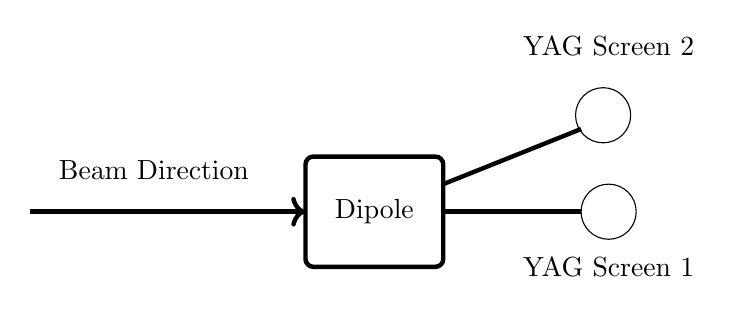
\begin{tikzpicture}[scale=0.7]
			
			\node[] at (2.25,0.75) {Beam Direction};
			\draw[ultra thick, ->] (0,0) -- (5.0, 0.0);
			
			\draw[fill=white, ultra thick, rounded corners =0.1cm] (5.0,1.0)rectangle  
			(7.5,-1.0) node[pos=0.5, align=center] {Dipole};
			
			\draw[ultra thick] (7.5, 0.0) -- (10.0, 0.0);
			\draw[ultra thick] (7.5, 0.5) -- (10.0, 1.5);
						
			\node[] at (10.5, 3) {YAG Screen 2};
			\draw (10.4,1.75) circle (0.5cm);
			
			\node[] at (10.5, -1.0) {YAG Screen 1};
			\draw (10.5,0) circle (0.5cm);
			
		\end{tikzpicture}
	\end{center} 
	\caption{Spectrometer set up in all cases at AWA.}
	\label{fig:spectrometer}
\end{figure*}

\Subsection{Energy Measurement Procedure}
Taking an energy measurement requires a beam trajectory
that is centered through the dipole. Otherwise, the beam 
may experience excessive non-uniform fields 
if it enters the dipole off-axis. The centering is done with two 
quads before the dipole. The center is found by focusing 
in the x-direction, and then the y-direction. If the beam 
moves to the left or the right as it is being focused, 
the quad is "steering", and the beam is entering the magnets off-axis.
Once the beam is centered through the quads on YAG screen 1, 
the dipole is then turned on to bend the beam.
The two YAG screens are positioned so that when the dipole is off, 
a centered beam will hit YAG screen 1. When the dipole is turned
on, the beam will appear at the center of YAG screen 2 when the 
beam is bent $20^\circ$. In this way, the dipole strength can 
then be used to determine the beam energy.

\Subsection{Energy Calculation}
Based on the procedure above, there is one number which we 
use to back calculate the mean energy. The amount of current
supplied to the dipole is represented by the number of "counts"
keyed into the control system. A counts to current line
is calculated given the measurements shown in Table \ref{tab:counts}
\begin{table}
\begin{center}
	\begin{tabular}{||c c||} 
		\hline
		Counts & Current [A] \\ [0.5ex] 
		\hline\hline
		1000 & 3.7 \\ 
		\hline
		5000 & 18.8 \\
		\hline
		10000 & 37.5 \\
		\hline
		15000 & 56.3 \\
		\hline
		
	\end{tabular}
\end{center}
\caption{Counts to current data for the first dipole in the drive beam line.}
\end{table}\label{tab:counts}
Then the B-field is calculated given the current: 
\begin{equation}
	\SI{}{B\,[T]} = (180.9708\cdot \SI{}{I\,[A]} - 7.2053)\cdot 10^{-4}
\end{equation}
There are a few geometric calculations that need to be done using the magnetic field value. 
before we can calculate the energy. 
The radius of curvature, $\rho$, 
can be calculated using the effective length of the dipole, L, and bending angle, $\theta$.
\begin{equation}
	\rho = \frac{L}{2\cdot \sin(\frac{\theta}{2})}
\end{equation}
Using $\rho$, and geometry, we can also estimate the x offset of the
beam after the dipole: 
\begin{equation}
	\Delta x = \rho \left( 1- \cos\theta \right)
\end{equation}
Using this and the famous relationship, $B\rho$ \cite{Wiedemann},
we can relate the B field and the beam momentum. 
\begin{equation}
	\SI{}{p\,\left[\frac{MeV}{c}\right]} = \frac{B\cdot \rho}{3.3356}\cdot 10^3
\end{equation}
We can then calculate the total energy by including the rest mass of the electrons \cite{Griffiths}:
\begin{equation}
	\SI{}{E\,[MeV]} = \sqrt{0.511^2+p^2}
\end{equation}\label{eq:energy}

\Subsubsection{Hard Edge Dipole Example}
\nrnote{this example is more of a double check and reference for me than for the reader...}
Since this calculation is used several time throughout the 
beam line for different magnets, lets consider a hard edge 
dipole, to show how the above equations can be used to determine
the x offset after the magnet, and the beam energy. 

Let's define the dipole length, $L=\SI{0.2}{[m]}$, angle, $\theta=\SI{20}{degrees}$. 
The corresponding radius is $\rho = \SI{0.5759}{[m]}$. With these values we can now 
calculate the offset, $\Delta x \approx \SI{34}{[mm]}$, which is confirmed by OPAL. 

\nrnote{not sure if I want to include energy since it depends on measured counts....}
Given a count of  energy of $\SI{64.8}{[MeV]}$ given measured counts of 

%%%%%%%%%%%%%%%%%%%%%%%%%%%%%%%%%%%%%%%%%%%%%%%%%%%%%%%%%%%%%%%%%%%%%%%%%%%%%%%%
%%%%%%%%%%%%%%%%%%%%%%%%%%%%%%%%%%%%%%%%%%%%%%%%%%%%%%%%%%%%%%%%%%%%%%%%%%%%%%%%
\Section{Transverse Beam Size Measurements} \label{sec:beamsize}
%%%%%%%%%%%%%%%%%%%%%%%%%%%%%%%%%%%%%%%%%%%%%%%%%%%%%%%%%%%%%%%%%%%%%%%%%%%%%%%%
%%%%%%%%%%%%%%%%%%%%%%%%%%%%%%%%%%%%%%%%%%%%%%%%%%%%%%%%%%%%%%%%%%%%%%%%%%%%%%%%
Beam size measurements are taken by using YAG screens at multiple z locations along the beam line.
The code used to produce all the following images can be found at this git repository:

\url{https://github.com/nneveu/imageProcessing}

\Subsection{Capturing Images}
\nrnote{Add tikz picture here to show how camera is pointed into beam line with mirrors}

\Subsection{Post Processing Images}
A python script was written to take beam images and convert them to profiles in the x and y direction.
This is done in a series of steps, and requires that one or more images can be used as a 
background image and fiducial image. A background image must capture any dark current 
that is present when the beam is not hitting the YAG screen. The fiducial image must 
clearly show the edges of the YAG screen so that a mm/pixel conversion can be calculated.
The following steps detail the post processing from raw image to transverse beam size estimate.

\Subsubsection{Step 1: Calculating the fiducial}

\Subsubsection{Step 2: Remove background intensity}

\Subsubsection{Step 3: Calculate x and y beam profile}

\Subsubsection{Step 4: Fit profile to calculate beam size}




%\Subsection{Kicker }
%%%%%%%%%%%%%%%%%%%%%%%%%%%%%%%%%%%%%%%%%%%%%%%%%%%%%%%%%%%%%%%%%%%%%%%%%%%%%%%%
%%%%%%%%%%%%%%%%%%%%%%%%%%%%%%%%%%%%%%%%%%%%%%%%%%%%%%%%%%%%%%%%%%%%%%%%%%%%%%%%
%\SubSection{Septum } 
%%%%%%%%%%%%%%%%%%%%%%%%%%%%%%%%%%%%%%%%%%%%%%%%%%%%%%%%%%%%%%%%%%%%%%%%%%%%%%%%
%%%%%%%%%%%%%%%%%%%%%%%%%%%%%%%%%%%%%%%%%%%%%%%%%%%%%%%%%%%%%%%%%%%%%%%%%%%%%%%%
\Chapter{Beam Dynamics}  
%%%%%%%%%%%%%%%%%%%%%%%%%%%%%%%%%%%%%%%%%%%%%%%%%%%%%%%%%%%%%%%%%%%%%%%%%%%%%%%%
%%%%%%%%%%%%%%%%%%%%%%%%%%%%%%%%%%%%%%%%%%%%%%%%%%%%%%%%%%%%%%%%%%%%%%%%%%%%%%%%
\Section{Code and Resources Used}\label{sec:code}
%%%%%%%%%%%%%%%%%%%%%%%%%%%%%%%%%%%%%%%%%%%%%%%%%%%%%%%%%%%%%%%%%%%%%%%%%%%%%%%%
%%%%%%%%%%%%%%%%%%%%%%%%%%%%%%%%%%%%%%%%%%%%%%%%%%%%%%%%%%%%%%%%%%%%%%%%%%%%%%%%

\lsnote{You need to start the chapter with summary paragraphs.  (1) Why are simulations needed?  (2) What simulation work was done?  (3) What method was chosen and why?  (4) What were the results?  You can't put  all of that in now, since some of it is unknown, but you should do (1), (3) and part of (2).  Also, before launching into the OPAL stuff, you need to say a few words about the beam characteristics during TBA studies.  A table of beam characteristics would be good here, one for the drive beam, and one for the witness.  After presenting the beam characteristics, you can mention that space charge is a problem for the drive beam - since now they know the intensity.}

With  the  rapid  improvement  in  computing  resources  and  codes  in  recent  years,  
accelerator  facilities  can  now achieve and rely on accurate beam dynamics simulations. 
These  simulations  include  single  particle  effects  (e.g. particle tracking in a magnetic field) as well as collective effects  such  as  space  charge  (SC),  
and  coherent  synchrotron  radiation  (CSR).

The beam dynamics reported in this thesis, were simulated with 
the open source, particle-in-cell (PIC) code OPAL was used \cite{opal}. 
PIC codes simulate the electromagnetic forces that particles see in an accelerator. 
This is done by mapping the input particles onto a grid. 
Then in each time (or z) step, the forces due to space charge, accelerating gradients, 
and magnets are calculated and applied to the grid.
OPAL comes in two flavors, OPAL-CYC and OPAL-T. The first is used to model 
cyclotrons, and the latter, which is used for this work, is suited for photoinjectors. 
OPAL-T was chosen in part because it models the 3D space charge necessary to accurately simulate the high charge bunches at the AWA. 
\lsnote{You need a few sentences describing OPAL.  Also describe (briefly) what a PIC code is.  (Are there any other choices besides a PIC code?)}
It was chosen for several reasons:
\begin{itemize}
	\item Able to calculate transverse space charge and wakefield forces 
	\item Option to run the code in parallel
	\item Data recorded in global and reference frames
\end{itemize} 

The first item is crucial to standard operations at the AWA. Especially in the 
case of TBA, high charge is needed on drive beam line, therefore transverse 
space charge must be calculated in the simulations to give realistic results.
The second item dramatically reduced the amount of simulation time needed. 
For example, simulating the gun and linac, about \SI{15}{m} of elements,
with 100,000 particles on one core would take about 30 minutes. 
When the number of cores is increased to 16, the same run takes less than 
5 minutes. This reduction in time by ~80\%, combined with the capability to run 
many cases at once on the cluster allows for more efficient use of time.
Typical running conditions were on 16 cores, for random samples up to 128 cores, 
and up to 5,200 cores for large optimization runs.  
\lsnote{Specifics are always good; do you have any numbers for the time for a parallel run versus single processor?  If not, it is not super important, but if those numbers are handy put them in.}

%%%%%%%%%%%%%%%%%%%%%%%%%%%%%%%%%%%%%%%%%%%%%%%%%%%%%%%%%%%%%%%%%%%%%%%%%%%%%%%%
%%%%%%%%%%%%%%%%%%%%%%%%%%%%%%%%%%%%%%%%%%%%%%%%%%%%%%%%%%%%%%%%%%%%%%%%%%%%%%%%
\Section{Benchmarking}
\nrnote{Copied and pasted NAPAC benchmark here, need to finish cleaning up.}
Using portions of AWA as the benchmark model,  
beam dynamics were simulated with three particle tracking codes.
The AWA rf photoinjector was benchmarked, primarily to study SC, 
in ASTRA, GPT, and OPAL-T using a \SI{1}{nC} beam. 
A $20^{\circ}$ dipole magnet was used to benchmark 
CSR effects in GPT and OPAL-T by bending a 1nC beam 
at  energies  between  2  MeV  and  100  MeV.  In  this  paper  
we  present  the  results,  and  discuss  the  similarities  and  
differences between the codes.
 
The AWA group has used several beam codes in the past including:
T-STEP/PARMELA~\cite{parmela}, ASTRA~\cite{astra}, and GPT~\cite{gpt}.  
In order to take advantage of computing resources offered by 
Argonne National Laboratory (ANL), an effort was made to investigate
OPAL~\cite{opal}, an open source and parallel code that comes in two flavors;  
OPAL-CYL and OPAL-T. The latter was installed on the Blues and Bebop clusters
at the Laboratory Computing Resource Center (LCRC) provided by ANL~\cite{lcrc}.
(See Appendix~\ref{build} for instruction on how to build OPAL-T at ANL.)

Since no members of AWA had prior experience with OPAL-T, a benchmark 
was done to compare \mbox{OPAL-T} results to the results of codes 
well known to the group (GPT and ASTRA). 
This ensured correct use of the code, and reliability of \mbox{OPAL-T}.
Two collective effects of interest to the AWA were used: 
space charge (SC) and coherent synchrotron radiation (CSR).
SC was tested using the drive gun at 1nC, and CSR was tested
using a hard edge dipole.


\Subsection{Gun Simulations}
The SC algorithms were probed using the AWA photoinjector, 
a 1.5 cell copper standing-wave cavity at 1.3 GHz, 
with bucking, focusing, and matching solenoids. 
In the remainder of this thesis, the word gun is used 
in place of photoinjector. The simulation parameters were chosen to 
approximately generate the canonical “\SI{1}{\micro\metre} at 1 nC” case.
The initial beam parameters were based on gun operations at PITZ \cite{pitz},
due to the similarities between the PITZ and AWA rf guns.
The PITZ parameters came close to achieving the \SI{1}{\micro\metre}
target without any optimization. A coarse 1D minimization
\nrnote{add method used here} of the 
emittance was done to determine the value of the laser radius 
used in this benchmark. The resulting minimum emittance was   
\SI{1.16}{\micro\metre}. 

The initial bunch distribution parameters as well as the 
on-axis gun gradient, and magnetic field used in 
the benchmark are listed in Table~\ref{tab:bench}. 
The rf gun and solenoid field maps were generated 
with the SUPERFISH/POISSON  codes~\cite{superfish}.
The gradient was chosen to match typical operations at PITZ~\cite{pitz}
and the AWA. The rf and solenoid fields seen by the beam in the gun are shown in Fig.~\ref{fig:gunfields}.
\begin{table}
	\begin{center}
		\begin{tabular}{l l} 
			\toprule
			\textbf{Parameter} & \textbf{Value} \\ 
			\midrule
			Charge & \SI{1}{nC} \\
			\addlinespace[-1em] 
			Gradient & \SI{60}{MV/m} \\
			\addlinespace[-1em] 
			Phase & Max energy (on crest) \\
			\addlinespace[-1em] 
			Laser radius & \SI{0.75}{mm} \\
			\addlinespace[-1em] 
			Rise and fall time & \SI{6}{ps} \\
			\addlinespace[-1em] 
			Initial kinetic energy & \SI{0.55}{eV} \\
			\addlinespace[-1em] 
			Matching solenoid strength & \SI{-0.389}{T} \\
			\addlinespace[-1em] 
			Buck and focusing solenoid strength & \SI{-0.12}{T} \\
			\bottomrule			
		\end{tabular}
	\end{center}
	\caption{Input simulation parameters for gun benchmark.}
\end{table}\label{tab:bench}
\begin{figure}
	\begin{center}
		\includegraphics[width=0.95\textwidth]{images/gun_EM_fields}\caption{Electric and magnetic fields seen by the beam on axis in the gun.}
	\end{center}
\end{figure}\label{fig:gunfields}

Note that the codes use various methods to model 
the rf and magnetic fields, SC, and image charge. 
The ASTRA simulations used the axial E field of the  
gun and solenoids, and then expanded the fields to find the
transverse components using the paraxial approximation 
(e.g. $E_r=-\frac{r}{2}\frac{dE_z}{dz}$). 
The simulations used a 2D cylindrical-symmetric SC algorithm with a uniform  
particle-deposition mesh; see ASTRA user manual~\cite{astra}.
The radial and longitudinal number of cells composing the mesh 
were $N_r=32$ and $N_z=64$, with 100k particles.  
The image charge close to the cathode was accounted for until 
the bunch reached \SI{9.7}{cm} from the cathode surface. 

GPT read in the 2D electric and magnetic field files,  
and used a square 3D adaptive SC mesh with $N_x=N_y=N_z=46$
with 100k particles, see spacecharge3Dmesh option in GPT manual~\cite{gpt}.
To calculate image charge, GPT uses a Dirichlet boundary condition at the  
cathode (z=0). The calculation is turned off when the  
distance between the beam and cathode is longer than the 
mesh box. OPAL-T also read in the field maps, and used a block 
structured equidistant SC mesh, see OPAL manual for SC calculation~\cite{opal}.  
Several square mesh sizes were run in OPAL-T. The results plotted in 
Fig.~\ref{fig:benchplot_gun} and~\ref{fig:benchplot_5m} correspond to a mesh of $N_x=N_y=N_z=46$, with 1 million particles. 
The image charge calculation uses a 
shifted integrated Green function \cite{imagecharge}.  
\begin{figure}
	\begin{center}
		\includegraphics[width=0.8\textwidth]{images/benchmark_gun}
		\caption{Beam envelopes in the gun.}
	    \label{fig:benchplot_gun}

        \vspace*{\floatsep}
        
		\includegraphics[width=0.8\textwidth]{images/benchmark_5m}
		\caption{Beam envelopes in drift.}
	    \label{fig:benchplot_5m}
	\end{center}
\end{figure}

In general, the simulation results are in reasonable agreement 
and within expectations based on previous benchmarks \cite{codecompare}. 
See Figs.~\ref{fig:benchplot_gun} and~\ref{fig:benchplot_5m} 
for beam envelopes in the gun and drift. 
The apparent disagreement of emittance between ASTRA and the other
two codes in the gun is because the former removes the angular momentum   
induced by the solenoid, while the later two codes do not. 
After the beam exits the solenoid, the emittance results  
are in good agreement, as shown in Fig.~\ref{fig:benchplot_5m}.

\Subsection{Dipole Simultaions}
Simulations  of  a  hard  edge  dipole  were  done  in  GPT  
and   OPAL-T   in   order   to   probe   CSR.   Short   
mono-energetic  Gaussian  bunches  with  zero  initial  emittance  
were sent through the dipole. Beam and dipole parameters 
are shown in Table~\ref{tab:benchcsr}. 
The CSR routine used in OPAL-T is based on 
the routine  used  in  ELEGANT  \cite{elegant}, which is known to assume  
the beam is ultra-relativistic. The CSR routine in GPT  
does  not  use  the  ultra-relativistic  approximation ($\beta=1$) 
and  as  a  result,  works  at  all energies  \cite{gptcsr}.  
Therefore, we expected  the  routines  to  match  well  at  high  energy  and  
diverge  at  lower  energy.  Results  of  the  CSR  simulations  
are  shown  in  Fig.  4.  As  expected,  the  results  between  
GPT and OPAL-T disagree at low energies. 
\begin{table}
	\begin{center}
		\begin{tabular}{l l} 
			\toprule
			\textbf{Parameter} & \textbf{Value} \\ 
			\midrule
			$\sigma_x =\sigma_y$ & \SI{1}{mm} \\
			\addlinespace[-1em] 
			Gradient & \SI{60}{MV/m} \\
			\addlinespace[-1em] 
			Phase & Max energy (on crest) \\
			\addlinespace[-1em] 
			Laser radius & \SI{0.75}{mm} \\
			\addlinespace[-1em] 
			Rise and fall time & \SI{6}{ps} \\
			\addlinespace[-1em] 
			Initial kinetic energy & \SI{0.55}{eV} \\
			\addlinespace[-1em] 
			Matching solenoid strength & \SI{-0.389}{T} \\
			\addlinespace[-1em] 
			Buck and focusing solenoid strength & \SI{-0.12}{T} \\
			\bottomrule			
		\end{tabular}
	\end{center}
	\caption{Input simulation parameters for gun benchmark.}
\end{table}\label{tab:benchcsr}


\Subsection{Convergence Study}
Convergence runs were done for three parameters: 
time step,  SC  mesh  size,  and  number  of  particles.  
Each  case was tested in the gun using the same field maps and 
baseline  settings  that  were  used  to  compare  SC  in  OPAL-T,  
ASTRA, and GPT. All OPAL-T simulations were run on 
16 cores, taking advantage of parallel calculations. 
The number of particles was varied from 20k to 3.2  million.  
The  longitudinal  parameters  (energy,  bunch length)  
showed  no  variation,  but  there  were  slight  deviations 
in the transverse emittance and beam size. The same results 
were observed when the time step was varied from 0.1 ps  to  10  ps.  
The  grid  size  was  changed  from  32,  44,  46, and 64 cubed; 
again the results lacked any major discrepancies.  
In all cases, no appreciable differences were observed in the energy,
emittance, beam size, or bunch length. In  most  cases,  
if unreasonable  parameters  were chosen, 
OPAL-T would not complete the run (crash or hang up).  

\nrnote{conclusion}
Based on the experience gained during this benchmark, 
all  three  codes  are  capable  of  accurate  simulations.  With  
respect  to  resources  at  the  AWA:  GPT  and  ASTRA  are  
better  suited  for  use  on  windows,  and  OPAL-T  is  better  
suited to Linux and parallel systems.

%At 40nC the usable gun phase range (for the 3D field map) is 
%$-30^\circ \le \phi_g \ge 30^\circ$. The usable region was defined 
%as the region where all particles are emitted from the gun. 
%i.e. at $40^\circ$, particles were lost. 
%%%%%%%%%%%%%%%%%%%%%%%%%%%%%%%%%%%%%%%%%%%%%%%%%%%%%%%%%%%%%%%%%%%%%%%%%%%%%%%%
%%%%%%%%%%%%%%%%%%%%%%%%%%%%%%%%%%%%%%%%%%%%%%%%%%%%%%%%%%%%%%%%%%%%%%%%%%%%%%%%
\Section{Optimization} \label{sec:opt}
Throughout the design process, optimization algorithms 
were used to shape the beam entering the TBA experimental area.
Minimizing the emittance and bunch length after the six cavity linac,
and choosing the optimal optics configuration for maximum beam transport 
were the main objectives of all optimization work.
The techniques used include model based, genetic,
and structure exploiting algorithms. 
 
Model-based, derivative-free, trust-region algorithms 
are increasingly popular for optimizing computationally 
expensive numerical simulations. A strength of such
methods is their efficient use of function evaluations. 
This was the first type of algorithm used to optimize 
the beam dynamics in two cases of interest at the AWA. 
First, the emittance of a \SI{1}{nC} electron 
bunch produced by the AWA rf photocathode gun 
was minimized by adjusting three parameters: rf gun phase, 
solenoid strength, and laser radius. The algorithm 
converges to a set of parameters that yield an
emittance of \SI{1.08}{\um}. Second, we expand 
the number of optimization parameters to model the complete AWA rf 
photoinjector (the gun and six accelerating cavities) at \SI{40}{nC}. 
The optimization algorithm was used in a Pareto study that compares the 
trade-off between emittance and bunch 
length for the AWA \SI{70}{MeV} photoinjector. \nrnote{finished?}

After a model based method was implemented, a common technique was 
used as confirmation and for exploratory work. Preliminary designs 
for the TBA optics configuration were probed using a Genetic Algorithm
that was built in to OPAL.  \nrnote{running simulations now}

Finally, to reduce the amount of time needed to optimize the complete beam line, 
a structure exploiting algorithm was implemented. \nrnote{working on this}


\Subsection{Bounded Optimization by Quadratic Approximation (BOBYQA)}
%\section{Optimization Algorithm}
% ----------------------------------------------------
Model-based, derivative-free algorithms are frequently used to optimize
computationally expensive simulations due to their judicious use of function
evaluations. In cases specific to accelerator physics, 
beam properties at different operational parameters are observed;
these methods then build models of the unknown
function and minimize these models to identify candidate parameters to 
evaluate. BOBYQA~\cite{bobyqa} is one such method that is available via the
NLopt~\cite{nlopt} package and was used in this study. 
Given a candidate set of optimal parameters $v^k$, BOBYQA
constructs a quadratic model using function values of points near $v^k$. 
This model is minimized in a neighborhood of $v^k$ in order to produce a point $\hat{v}$. If $\hat{v}$ has a smaller objective function value than $v^k$, 
the estimate of the optimum is updated to $\hat{v}$, and a new model is constructed. 
If $\hat{v}$ is not a sufficient improvement over $v^k$, 
the model around $v^k$ is improved. For more
information about derivative-free optimization, see~\cite{Conn2009a}.

The parameters $v^k$ are generated and supplied to OPAL\=/T~\cite{opal}. 
The optimization package NLopt and OPAL\=/t were used
in combination with Python code written at ANL with the help 
of Jeff Larson, to perform simulation evaluations and optimization.
All the files needed to replicate the results in this section are available at
\begin{center}
	www.mcs.anl.gov/$\sim$jlarson/AWA
\end{center}
Interested parties are welcome to adapt the code to their needs
and suggest improvements.

\Subsection{Optimization Parameters}
% ----------------------------------------------------
When optimizing the gun, three parameters were varied: 
solenoid strength ($S_3$), gun phase ($\phi_g$), 
and laser radius ($R$) of a uniform pulse. 
The minimized objective was emittance ($\epsilon_x$).
(The phase is defined as $0^{\circ}$ at maximum energy gain.) 
When optimizing the entire linac, seven additional parameters were 
varied: the longitudinal laser full width at half maximum ($T$)
and accelerating cavity phases ($\phi_L$). The optimization parameters and
bounds are given in table~\ref{tab:parameters}; we denote the set of
ten optimization parameters as $v=[S_3, \phi_g, R, T, \phi_L]$, where 
$\phi_L=[\phi_{L_1},\ldots,\phi_{L_6}]$ represents the phase of each linac cavity $L_1$-$L_6$. 
\nrnote{need to fix footnotes and superscripts for table 3.3}
\begin{table}
	\caption{\label{tab:parameters} Parameter bounds for gun and linac optimization.}
	\begin{center}
		\begin{tabular}{ l *{3}{c}} 
			\toprule
			\textbf{Variable} & \textbf{Range} & \textbf{Unit} \\
			\midrule
			Solenoid Strength & $ 0 \le S_3 \le 440$  & amps \\
			Phase of Gun & $-60 \le \phi_g \le 60$  & degrees \\
			Laser Radius  & $0.1 \le R \le 30$  & mm \\
			Laser FWHM \footnotemark \label{note1}& $2 \le T \le $10  & ps \\
			Cavity Phase \textsuperscript{\ref{note1},}\footnotemark & $-20 \le \phi_L \le 20$  & degrees \\
			\bottomrule	
		\end{tabular}
	\addtocounter{footnote}{-1}\footnotetext{not varied during gun optimization}
	\addtocounter{footnote}{+1}\footnotetext{$\phi_L=[\phi_{L_1},\ldots,\phi_{L_6}]$}
	\end{center}
\end{table}


\Subsection{Gun Simulations Using BOBYQA} \label{sec:gunbobyqa}
%\section{Gun Optimization}
% ----------------------------------------------------
Much work has been done to optimize 1.5 cell rf guns
at \SI{1}{nC}~\cite{pitz}. This known solution was used as 
a baseline test of BOBYQA when applied to an accelerator application.
An optimization of the single objective emittance ($\epsilon_x$) was 
performed over a length of \SI{5}{m}. 
All linacs were turned off and only gun parameters were varied. 
Non-varying parameters are listed in table~\ref{tab:gun}; 
their values are based on work done at PITZ and AWA~\cite{pitz, benchmark}.

Local optimization runs were started from five points with various distances from the optimum value. The optimization runs converged 
(in less than 100 function evaluations) to a parameter set ($S_3=\SI{269}{A}$, $\phi_g=\SI{-3.0}{^{\circ}}$, and $R=\SI{0.6}{mm}$) 
with an emittance of $\SI{1.08}{\um}$.
An exhaustive search of the parameter space was not done, and there may be other local minima that were not found.
However, the results match expectations based on the literature. 
\begin{table}[h] 
	\caption{\label{tab:gun} Non-varying parameters for gun optimization.}
	\begin{center}
		\begin{tabular}{lll}
			\toprule
			\textbf{Parameter} & \textbf{Value} \\
			\midrule
			Charge  & \SI{1}{nC} \\
			Gradient & \SI{60}{MV/m} \\
			Laser FWHM & \SI{20}{ps} \\
			Laser Rise and Fall Time & \SI{6}{ps} \\
			Kinetic Energy at Cathode  & \SI{0.55}{eV} \\
			$S_1$ and $S_2$ & \SI{550}{A} \\
			\bottomrule
		\end{tabular}
	\end{center}
\end{table}


\Subsection{Linac Description} \label{sec:pareto}
\nrnote{maybe this beam line description should be in chp 2:
The \SI{70}{MeV} rf photoinjector at the AWA
consists of an rf gun followed by six rf accelerating cavities, 
hereafter referred to as the linac. 
See Figure~\ref{fig:beamline} for the beam line layout. 
The 1.5 cell rf gun operates at \SI{1.3}{GHz} with three solenoids 
and a Cs$_{2}$Te photocathode excited by a \SI{248}{nm} UV laser.  
Solenoid 1 ($S_1$) is used to buck the field at the cathode,
while the other two solenoids ($S_2$ and $S_3$) are used for emittance compensation.  
The accelerating cavities, also operated at \SI{1.3}{GHz}, are 7 cell standing-wave 
cavities \cite{Power:2010zza} each with independently controllable phase. 
The cavities are labeled $L_1$-$L_6$ in Figure~\ref{fig:beamline}. }
\def \gunleft {-1.0}
\def \gunright {0.3}
\def \loneright {1.0}
\def \ltworight {3.5}
\def \lthreeright {5.0}
\def \lfourright {7.0}
\def \lfiveright {8.5}
\def \lsixright {10}
\begin{figure*}
	\captionsetup{width=0.98\linewidth}
	\begin{center}
		
		\begin{tikzpicture}[scale=0.95]
		%Gun drawings
		\draw[fill=orange, very thick, rounded corners =0.1cm] (\gunleft,0.5)rectangle (\gunright,1.5) node[pos=.5, white] {\textbf{Gun}} ;
		
		%S1
		\node[] at (-1.3,2.9) {$S_1$};
		\draw[ultra thick, fill=black!60!green] (-1.4,-0.5)rectangle  (-1.0,0.5) node[pos=.5, white] {} ;
		\draw[black, ultra thick] (-1.4,-0.5) -- (-1.0,0.5);
		\draw[black, ultra thick] (-1.4,0.5) -- (-1.0,-0.5);
		\draw[ultra thick, fill=black!60!green] (-1.4,1.5)rectangle  (-1.0,2.5) node[pos=.5, white] {} ;
		\draw[black, ultra thick] (-1.4,1.5) -- (-1.0,2.5);
		\draw[black, ultra thick] (-1.4,2.5) -- (-1.0,1.5);
		%S2
		\node[] at (-0.8,2.9) {$S_2$};
		\draw[ultra thick, fill=black!60!green] (-1.0,-0.5)rectangle  (-0.6,0.5) node[pos=.5, white] {} ;
		\draw[black, ultra thick] (-1.0,-0.5) -- (-0.6,0.5);
		\draw[black, ultra thick] (-1.0,0.5) -- (-0.6,-0.5);
		\draw[ultra thick, fill=black!60!green] (-1.0,1.5)rectangle  (-0.6,2.5) node[pos=.5, white] {} ;
		\draw[black, ultra thick] (-1.0,1.5) -- (-0.6,2.5);
		\draw[black, ultra thick] (-1.0,2.5) -- (-0.6,1.5);
		
		%S3
		\node[] at (0.2,2.9) {$S_3$};
		\draw[ultra thick, fill=black!60!green] (-0.1,-0.5) rectangle  (0.3,0.5) node[pos=.5, white] {};
		\draw[black, ultra thick] (-0.1,-0.5) -- (0.3,0.5);
		\draw[black, ultra thick] (-0.1,0.5) -- (0.3,-0.5);
		\draw[ultra thick, fill=black!60!green] (-0.1,1.5) rectangle  (0.3,2.5) node[pos=.5, white] {};
		\draw[black, ultra thick] (-0.1,1.5) -- (0.3,2.5);
		\draw[black, ultra thick] (-0.1,2.5) -- (0.3,1.5);
		%Linac drawings 
		\draw[fill=blue, ultra thick, rounded corners =0.1cm] (\loneright,0)rectangle  ({\loneright+0.84},2) node[pos=.5, white] {$L_1$} ;
		\draw[fill=blue, ultra thick, rounded corners =0.1cm] (\ltworight,0)rectangle  ({\ltworight+0.84},2) node[pos=.5, white] {$L_2$};
		\draw[fill=blue, ultra thick, rounded corners =0.1cm] (\lthreeright,0)rectangle ({\lthreeright+0.84},2) node[pos=.5, white] {$L_3$};
		\draw[fill=blue, ultra thick, rounded corners =0.1cm] (\lfourright,0)rectangle ({\lfourright+0.84},2) node[pos=.5, white] {$L_4$};
		\draw[fill=blue, ultra thick, rounded corners =0.1cm] (\lfiveright,0)rectangle ({\lfiveright+0.84},2) node[pos=.5, white] {$L_5$};
		\draw[fill=blue, ultra thick, rounded corners =0.1cm] (\lsixright,0)rectangle ({\lsixright+0.84},2) node[pos=.5, white] {$L_6$};
		\draw[very thick] (\gunleft,-1.5) -- (14,-1.5);
		\draw[latex-latex] (\gunleft,-1.5) -- (14,-1.5) ; 
		\foreach \x in  {0.3, 1.0, 3.5, 5.0, 7.0, 8.5, 10, 12.5} %tick marks
		\draw[shift={(\x,-1.5)},color=black] (0pt,3pt) -- (0pt,-3pt);
		\foreach \x in {0.3, 1.0, 3.5, 5.0, 7.0, 8.5, 10, 12.5}
		\draw[shift={(\x,-1.7)},color=black] (0pt,0pt) node[below] 
		{$\x$};
		
		\node[draw, fill=yellow, star, star points=5, star point ratio=0.6, minimum size=0.6cm]
		at (12.5,1.0) {$z_1$};
		\end{tikzpicture}
	\end{center}
	\caption{Layout of the AWA linac.
		The gun is enlarged to show solenoid detail. The physical length is
		\SI{0.3}{m}. The cathode is located at $z=\SI{0}{m}$. Linac cavities are
		\SI{0.85}{m} long. Tick marks are located at the exit of the gun, entrance of
		each accelerating cavity, and location of optimization.}
	\label{fig:beamline} 
\end{figure*} 

\Subsection{Linac Optimization}
%\section{Linac Optimization} 
% ----------------------------------------------------
Next we performed a multiobjective optimization of the linac (Figure~\ref{fig:beamline}), 
by adjusting the ten parameters in table~\ref{tab:parameters}. The charge was set to \SI{40}{nC}
and was chosen for upcoming two-beam acceleration experiments~\cite{tba2017}. 
Two objectives were considered: emittance, and bunch length, $\sigma_z$. 
The location of interest is $z_1=\SI{12.51}{m}$, as this is the entrance of the first 
quadrupole magnet after the linac. We optimize $\epsilon_x$ instead of $\epsilon_{xy}$ because 
no asymmetric focusing elements were used in the linac. 
The non-varying parameters for all linac simulation runs are shown in table~\ref{tab:linac}.
The model used simulated emission
from a Cs$_2$Te cathode using a laser with initial kinetic energy of \SI{4}{eV}. 
These are typical operating conditions at AWA. 
\begin{table}[h] %or [hbt] ?
	\caption{\label{tab:linac} Non-varying parameters for linac optimization.}
	\begin{center}
		\begin{tabular}{lll}
			\toprule
			\textbf{Parameter} & \textbf{Value} \\
			\midrule
			Charge  & \SI{40}{nC} \\
			Laser Rise and Fall Time & \SI{1.0}{ps} \\
			Gun Gradient & \SI{70}{MV/m} \\
			$S_1$ and $S_2$ & \SI{550}{A}\\
			Cavity Gradient $L_1$--$L_4$ & \SI{25}{MV/m} \\
			Cavity Gradient $L_5$--$L_6$ & \SI{27}{MV/m} \\
			\bottomrule
		\end{tabular}
	\end{center}
\end{table}

A 1,000 point sample of linac parameters were drawn from the domain
in table~\ref{tab:parameters} and simulated. Of these, 132 simulations completed
without error, and the emittance and bunch length at $z_1=\SI{12.51}{m}$ was
recorded for each of these points. From the sample, the minimum and maximum values of emittance and bunch length
were found (i.e: $\epsilon_{\min}$ and $\epsilon_{\max}$). 
The raw $\epsilon_x(v,z_1)$ and $\sigma_z(v,z_1)$ sample values were then
shifted and scaled to produce $\bar{\epsilon}_x(v,z_1)$, and $\bar{\sigma}_z(v,z_1)$,
which have a minimum value of 0 and a maximum value of 1 over the 132-point sample set. That is, 
\begin{equation}
\bar{\epsilon}_x (v,z_1) = \frac{ \epsilon_x (v,z_1) - \epsilon_{\min} } { \epsilon_{\max} - \epsilon_{\min} }
\label{eq:scale}
\end{equation} 
and $\bar{\sigma}_z (v,z_1)$ is defined similarly.
This scaling is done in order to remove the difference in the units between
emittance and bunch length when optimizing.

With the scaled values of $\bar{\epsilon}_x$ and $\bar{\sigma}_z$, a sequence
of eleven optimization problems were solved by minimizing,
\begin{equation}
f(v,w) = w \,\bar{\epsilon}_x(v,z_1) + (1-w)\, \bar{\sigma}_z(v,z_1)
\label{eq:newobj}
\end{equation}
for $w \in \left\{ 0, 0.1, \ldots, 1 \right\}$. 
For each weight $w$, BOBYQA was started from the sample point with the 
smallest value of $f(v,w)$.  From the initial random sample, six unique starting points were chosen. 
(There were fewer starting points than weights because some samples had the smallest objective value for multiple weights. 
For example, the smallest values of $f(v,0.4)$, $f(v,0.5)$, and $f(v,0.6)$ occurred when at the eighteenth sample point.)
Some $f(v,w)$ values also had one or more linac phases near the initial $\pm20^{\circ}$ boundary. 
The $\phi_L$ boundary was expanded to $\pm40^{\circ}$ for those BOBYQA runs.

\Subsection{Pareto Front for AWA Linac}
%\section{Pareto Front for AWA Linac} 
% ----------------------------------------------------
Since multiple objectives are under consideration in this case, a
trade-off analysis is necessary. 
\begin{figure}[h]
	\captionsetup{width=0.98\linewidth}
	\begin{center}
		\includegraphics[width=0.98\textwidth]{images/THPAB155f1}
		\caption{Random sample results, starting sample points, and resulting approximate Pareto front for the linac at \SI{40}{nC}. The Pareto front is the result of all BOBYQA evaluations.}
		\label{fig:pareto}
	\end{center}
\end{figure}
This can be aided by examining a Pareto front: the set of parameters 
for which no other point exists that is better with respect to both objectives~\cite{ehrgott2006multicriteria}.
In Figure~\ref{fig:pareto}, blue dots show the emittance and bunch length for the
evaluated random sample. The sample points for which no other point has better
emittance and bunch length are connected with a blue line. BOBYQA was started
from these points, as described above, producing the green approximate Pareto front. 


The number of simulation evaluations needed to obtain convergence
in the BOBYQA runs varied from a minimum of 107 evaluations to a maximum of 208 
evaluations. In order to generate the Pareto front in
Figure~\ref{fig:pareto}, a total of 2,492 simulation evaluations were completed.
Most simulation evaluations took approximately 7 minutes, using 16 cores and 100,000 particles. These numbers are driven by the amount of time OPAL-T needs to simulate the beam line. 

The best-found objective value through each BOBYQA run is shown in Figure~\ref{fig:iterations}. 
Weight 0.0 and 1.0 are negative due to the scaling in Equation~(\ref{eq:scale}). While the weights, $w$, are always nonnegative, 
$\bar{\epsilon}_x (v,z_1)$ or $\bar{\sigma}_z(v,z_1)$ will be negative if BOBYQA finds a point with a value of 
$\epsilon_x(v,z_1)$ or $\sigma_z(v,z_1)$ that is less than $\epsilon_{\min}$ or $\sigma_{\min}$ from the initial sample. 
\begin{figure}[h]
	\captionsetup{width=0.98\linewidth}
	\begin{center}
		\includegraphics[width=0.98\textwidth]{images/THPAB155f2}
		\caption{\label{fig:iterations}Minimum observed objective function values during eleven BOBYQA runs at \SI{40}{nC}.}
	\end{center}
\end{figure}

We note that seven of the BOBYQA runs converged to emittance values
between \SI{20}{\mu m} and \SI{50}{\mu m}, which is shown in Figure~\ref{fig:trade} 
along with gun phase and bunch length for each of the 11
optimized points. We annotate Figure~\ref{fig:trade} with $T$ because that parameter 
shows strong correlation with the gun phase. Other optimized parameters such as the laser radius were found to stay within a 
narrow range (\SIrange{10}{16}{mm}).  
\begin{figure}[h]
	\captionsetup{width=0.98\linewidth}
	\begin{center}
		\includegraphics[width=0.98\textwidth]{images/THPAB155f3}
		\caption{\label{fig:trade}Bunch length and emittance vs.~gun phase at each optimized point in the Pareto front for the linac at \SI{40}{nC}. The phase of the max energy gain is 0$^{\circ}$.}
	\end{center}
\end{figure}


The optimized linac phases maximize energy gain while minimizing the energy spread.
The energy spread of the beam exiting the gun depends strongly on $\phi_g$.
There are three distinct regions where the optimized points had similar gun phases 
(less than $\pm10^{\circ}$) which resulted in nearly identical linac phases. For example:  
all six phases, $\phi_L$, varied by less than $10^{\circ}$ for $w \in \left\{ 0, 0.1\right\}$,
less than $5^{\circ}$ for $w \in \left\{ 0.4, 0.5, 0.6\right\}$, 
and less than $10^{\circ}$ for $w \in \left\{ 0.7, 0.8, 0.9\right\}$.
This indicates optimized linac phases may benefit a range of gun settings during operation. 


\Subsection{Lessons Learned from BOBYQA Work}
\nrnote{conclusion from paper... add some?}
% ----------------------------------------------------
Using an AWA beam line as the simulation model, we used the BOBYQA algorithm 
to optimize the emittance produced by the gun at \SI{1}{nC}.
Using the same algorithm, we performed a multiobjective analysis for the linac at \SI{40}{nC}. 
A Pareto front comparing the trade-off between bunch length and emittance was generated for the linac. 
In total, only 2,492 simulation evaluations were needed to produce the approximate Pareto front.
From this work a few key take aways are clear. First, larger laser radius
is uniformly better for high charge. i.e large radius helps lower emittance.
The second clear results is alternating the phases in the linac can control 
the energy spread created by the gun, i.e. running off crest in the linac 
can reduce the energy spread significantly.

%%%%%%%%%%%%%%%%%%%%%%%%%%%%%%%%%%%%%%%%%%%%%%%%%%%%%%%%%%%%%%%%%%%%%%%%%%%%%%%%
%%%%%%%%%%%%%%%%%%%%%%%%%%%%%%%%%%%%%%%%%%%%%%%%%%%%%%%%%%%%%%%%%%%%%%%%%%%%%%%%
\Section{OPAL and the Genetic Algorithm: NSGA-II} \label{sec:ga}
%%%%%%%%%%%%%%%%%%%%%%%%%%%%%%%%%%%%%%%%%%%%%%%%%%%%%%%%%%%%%%%%%%%%%%%%%%%%%%%%
%%%%%%%%%%%%%%%%%%%%%%%%%%%%%%%%%%%%%%%%%%%%%%%%%%%%%%%%%%%%%%%%%%%%%%%%%%%%%%%%
Next, work began on designing the TBA experimental area. 
Initial probes into this problem were done using the genetic algorithm
implemented in OPAL-T~\cite{optpilot}.


%%%%%%%%%%%%%%%%%%%%%%%%%%%%%%%%%%%%%%%%%%%%%%%%%%%%%%%%%%%%%%%%%%%%%%%%%%%%%%%%
%%%%%%%%%%%%%%%%%%%%%%%%%%%%%%%%%%%%%%%%%%%%%%%%%%%%%%%%%%%%%%%%%%%%%%%%%%%%%%%%
%\Section{Kicker}




%%%%%%%%%%%%%%%%%%%%%%%%%%%%%%%%%%%%%%%%%%%%%%%%%%%%%%%%%%%%%%%%%%%%%%%%%%%%%%%%
%%%%%%%%%%%%%%%%%%%%%%%%%%%%%%%%%%%%%%%%%%%%%%%%%%%%%%%%%%%%%%%%%%%%%%%%%%%%%%%%
\Section{Kicker Design}

\lsnote{You need to start with a re-statement of the purpose of the kicker. }
A design implemented by Indiana University (IU) \cite{iukicker}
will be adapted to fit TBA requirements at the AWA. Redesign will require optimization
of the length and gap between the kicker plates. \lsnote{Summarize what criteria are used to determine these.} Figure \ref{fig:IUkicker} shows the existing IU kicker.
\begin{figure}[h]
	\begin{center}
		%\includegraphics[scale=0.5]{C:/Users/nneveu/Pictures/kicker.jpg}\caption{IU Kicker \cite{IUkicker}}
		\label{fig:IUkicker}
	\end{center}
\end{figure}
The kicker is essentially a parallel plate waveguide. 
A $\pm$35 kV power supply will be used to induce a 70 kV potential difference 
across the plates. Each plate will be terminated in a 50 $\Omega$ load to induce a steady 
state current on the plates. The combination of the two will result in a static TEM mode 
between the plates. Calculation of the electric, $E_v$, and magnetic field, $B_v$,
can be derived from the voltage or current. The electric field, $E_v$, due to a potential, V, is: 
\begin{equation}
E_v=\frac{V}{h}
\end{equation}

Where h is the gap height. From Maxwell's equations, we know that the electric and magnetic 
field are related by the speed of light, c, in the case of plane and TEM waves \cite{pozar}. 
From this we can find the magnetic field induced between the plates: 
\begin{equation}
B_v=\frac{E_v}{c}
\end{equation}
The electrons are going at the speed of light, $c$, and are moving through the kicker on a 
trajectory perpendicular to the fields.  So, it can be seen from the Lorentz force equation, that the force 
exerted on a charge q from the electric and magnetic fields of the TEM mode are equal. 
\begin{equation}
F=q(E_v+v\times B_v)
\end{equation}

Since the force due to the electric field is equal and in the same direction as that from the magnetic field, 
the total kick is just twice that from either field alone.  The angle induced by each field is \cite{iukicker, Wiedemann}:  
\begin{equation}
\theta_E= \frac{V\,L}{h\,T}
\end{equation}
\begin{equation}
\theta_B= \frac{B\,L}{B\rho}
\end{equation}

Where L is the plate length, and T is the kinetic energy of the beam. $B\rho=3.33564\,*T\,$ [GeV-Tesla] is a 
common accelerator physics term that can be found in text such as Wiedemann \cite{Wiedemann}. 
The total angle provided by the kicker is then: 
\begin{equation}
\theta_{total}= \theta_E+\theta_B=2\theta_E=2\theta_B
\end{equation}
From these equations, variable parameters include the gap height, length of the plates, and 
the kinetic energy of the beam. The largest drive beam energy achievable at the AWA is 75 MeV. 
Thesis work will include the optimization of these parameters to obtain the largest angle possible.
Simulations have begun to set boundary conditions on the variable parameters. 



\Chapter{Experimental Measurements}%________________________________

\Chapter{Experimental Results} 
%%%%%%%%%%%%%%%%%%%%%%%%%%%%%%%%%%%%%%%%%%%%%%%%%%%%%%%%%%%%%%%%%%%%%%%%%%%%%%%%%%%%%%%%%%%%
%%%%%%%%%%%%%%%%%%%%%%%%%%%%%%%%%%%%%%%%%%%%%%%%%%%%%%%%%%%%%%%%%%%%%%%%%%%%%%%%%%%%%%%%%%%%
\Section{Measurement of Single Stage Power Extraction}
%%%%%%%%%%%%%%%%%%%%%%%%%%%%%%%%%%%%%%%%%%%%%%%%%%%%%%%%%%%%%%%%%%%%%%%%%%%%%%%%%%%%%%%%%%%%
%%%%%%%%%%%%%%%%%%%%%%%%%%%%%%%%%%%%%%%%%%%%%%%%%%%%%%%%%%%%%%%%%%%%%%%%%%%%%%%%%%%%%%%%%%%%
%\Section{Measurement of Single Stage Accelerating Gradient}
%\Section{Measurement of Staged Two Beam Acceleration}

\footnote{My Footnote} 
\Chapter{CONCLUSION}
%   \input{Conclusion.tex}
You need a Conclusion.tex file

\Section{Summary}


This was just to create a sample section...

\clearpage


%
% APPENDIX
%
\appendix

\Appendix{How to build OPAL on Bebop at ANL} \label{build}
This set of instructions is tailored to the bebop cluster at ANL. 
Intel compilers and intel-MPI were used to build OPAL and all 
the libraries it is dependent on.
\begin{enumerate}[label=Step \arabic*:]
	\item Load modules 

I purge modules first, this will force an error message if any changes
to the system modules occur.
\begin{lstlisting}
	module purge
	module load intel
	module load intel-mpi 
	module load cmake 
	module load gmp   
	module load mpfr  
	module load mpc   
	module load hdf5   
	module load gsl   
	module load intel-mkl
	module load szip
\end{lstlisting}

    \item Set environment variables for compilers 
 
These variables point to intel compilers. 
\begin{lstlisting}
CC=mpiicc;CXX=mpiicpc;F90=ifort;F77=ifort
export CC CXX F90 F77
\end{lstlisting}

    \item Set enviornment variables for self built libraries.
    
I built these libraries separately because they were not available as 
modules on the cluster. 

\begin{lstlisting}
	export PATH="/blues/gpfs/home/neveu/git/H5hut-2.0.0rc3/build:${PATH}"
	
	export H5HUT_HOME=$HOME/git/H5hut-2.0.0rc3/build_intel
	export H5HUT_PREFIX=$H5HUT_HOME
	export H5HUT_DIR=$H5HUT_HOME
	export H5HUT_INCLUDE_DIR=$H5HUT_HOME/include
	export H5HUT_LIBRARY_DIR=$H5HUT_HOME/lib
	
	export BOOST_HOME=$HOME/git/boost_1_62_0/build/
	export BOOST_DIR=$BOOST_HOME
	export BOOST_PREFIX=$BOOST_HOME
	export BOOST_INCLUDE_DIR=$BOOST_HOME/include
	export BOOST_LIBRARY_DIR=$BOOST_HOME/lib
	export BOOST_ROOT=/home/neveu/git/boost_1_62_0/
	echo $BOOST_ROOT
	echo $BOOST_DIR
\end{lstlisting}

    \item Call cmake 
    
There are two cmake calls I use depending on if I'm building for 
BDW (\verb|-axCORE-AVX2|) or KNL (\verb|-axMIC-AVX512|) architecture. 
    
\begin{lstlisting}
cmake -DCMAKE_INSTALL_PREFIX=/home/neveu/software/opal-1.9/bdw -DCMAKE_CXX_FLAGS="-lsz -axCORE-AVX2" ..
\end{lstlisting}

    \item Call make, then make install
I usually call make with a large number of cores to speed up the compilation.    
\begin{lstlisting}
	make -j 30 
	make install
\end{lstlisting}

\end{enumerate}



%\moretox

\Appendix{OPAL stuff? MCS Stuff?}

Your second appendix text....

\newpage
%
% BIBLIOGRAPHY
%
\bibliographystyle{plain}
\bibliography{thesis}

\end{document}  % end of document





























